%%%%%%%%%%%%%%%%%%%%%%%%%%%%%%%%%%%%%%%%%
% Focus Beamer Presentation
% LaTeX Template
% Version 1.0 (8/8/18)
%
% This template has been downloaded from:
% http://www.LaTeXTemplates.com
%
% Original author:
% Pasquale Africa (https://github.com/elauksap/focus-beamertheme) with modifications by 
% Vel (vel@LaTeXTemplates.com)
%
% Template license:
% GNU GPL v3.0 License
%
% Important note:
% The bibliography/references need to be compiled with bibtex.
%
%%%%%%%%%%%%%%%%%%%%%%%%%%%%%%%%%%%%%%%%%

%----------------------------------------------------------------------------------------
%	PACKAGES AND OTHER DOCUMENT CONFIGURATIONS
%----------------------------------------------------------------------------------------

\documentclass{beamer}

\usepackage[absolute,overlay]{textpos}
\usepackage{media9}
\usepackage{hyperref}

\usetheme{focus} % Use the Focus theme supplied with the template
% Add option [numbering=none] to disable the footer progress bar
% Add option [numbering=fullbar] to show the footer progress bar as always full with a slide count

% Uncomment to enable the ice-blue theme
\definecolor{main}{RGB}{92, 138, 168}
\definecolor{background}{RGB}{240, 247, 255}

\title{Reinforcement Learning}

% A subtitle is optional and this may be deleted
\subtitle{Atari Games}

\author{Isabell Lederer\\
\small \textsc{github.com/mathebell/RL\_Atari\_Games}}
% - Give the names in the same order as the appear in the paper.
% - Use the \inst{?} command only if the authors have different
%   affiliation.

\institute[TU Wien] % (optional, but mostly needed)
{AKNUM Maschinelles Lernen SE}
% - Use the \inst command only if there are several affiliations.
% - Keep it simple, no one is interested in your street address.

\date{Wien, 18. Dezember 2018}
% - Either use conference name or its abbreviation.
% - Not really informative to the audience, more for people (including
%   yourself) who are reading the slides online

\titlegraphic{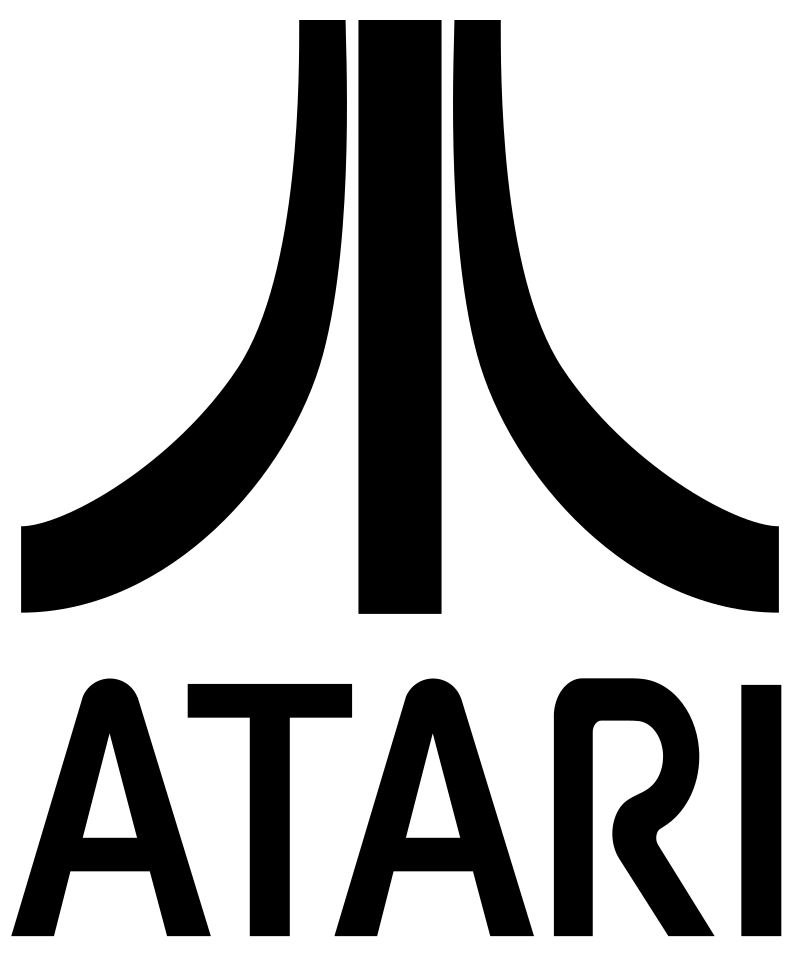
\includegraphics[scale=0.1]{Images/atari_logo}}

\begin{document}

\begin{frame}
  \titlepage
\end{frame}
%--------------------------------------------------------------------
\begin{frame}{Overview}
			Contents:
			\begin{enumerate}
				\item Introduction
				\begin{enumerate}
					\item Atari Games
					\item New Problem
				\end{enumerate}
				\item The mathematics behind the algorithm
				\begin{enumerate}
					\item Q-learning and DQN
					\item Policy Gradient Methods and Theorem
					%\item Actor-critic Methods
				\end{enumerate}
				\item Implementation
				\begin{enumerate}
					\item Preprocessing
					\item Model architecture
					\item Pseudocode DQN
				\end{enumerate}
				\item Results
				\begin{enumerate}
					\item Video clip
					\item Performance
				\end{enumerate}
				

			\end{enumerate}
\end{frame}
%--------------------------------------------------------------------
\begin{frame}{Atari Games}

\begin{columns}
	\column{0.5\textwidth}
	\centering
	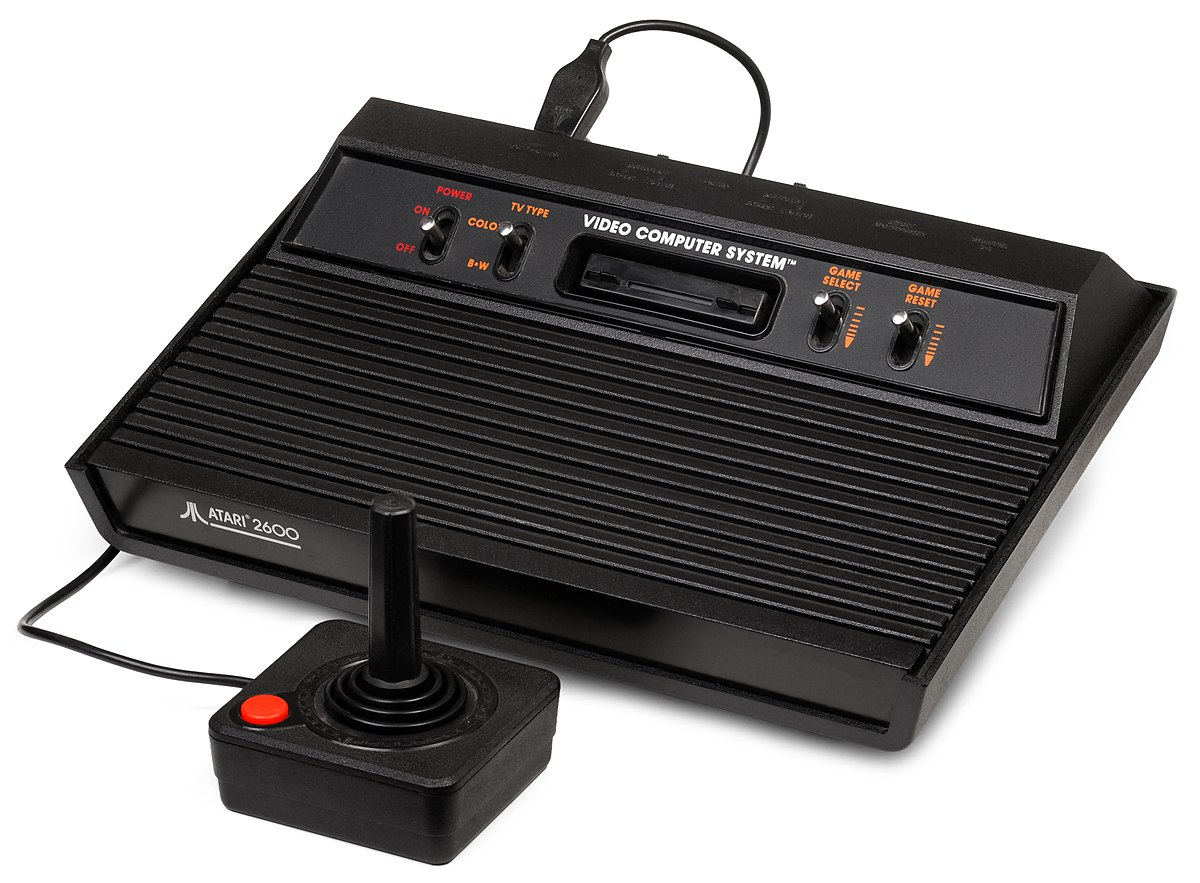
\includegraphics[scale = 0.15]{Images/Atari-2600-Console.jpg}

\column{0.5\textwidth}
\centering
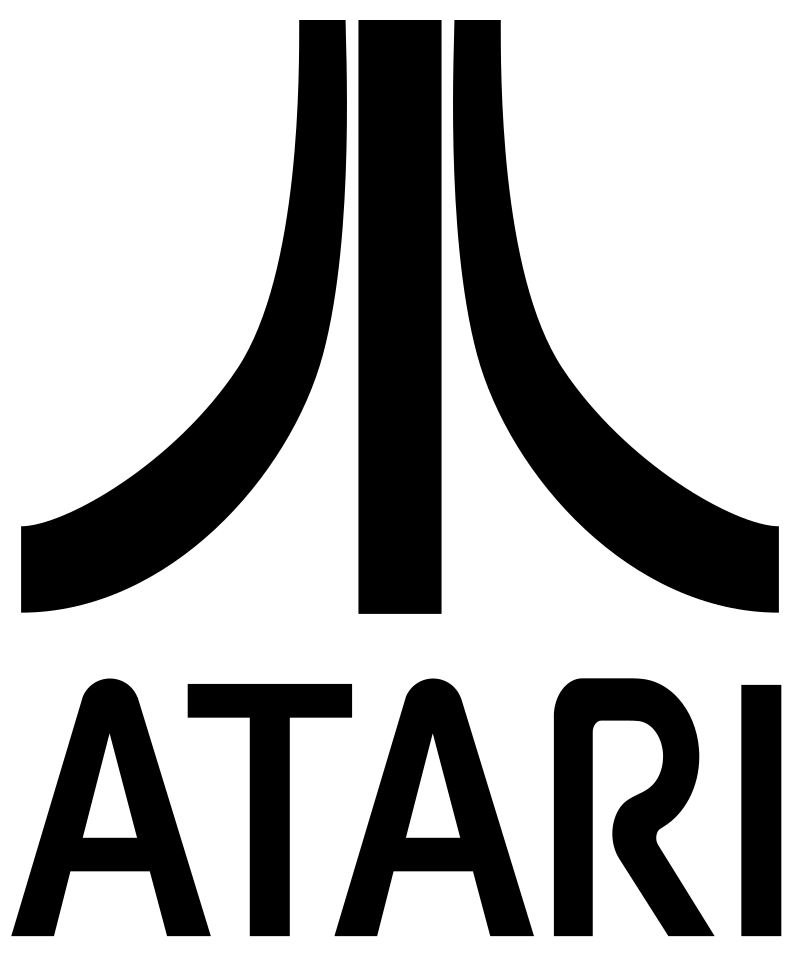
\includegraphics[scale = 0.1]{Images/atari_logo}
\end{columns}

\end{frame}
%--------------------------------------------------------------------
\begin{frame}{Atari Games}
\centering
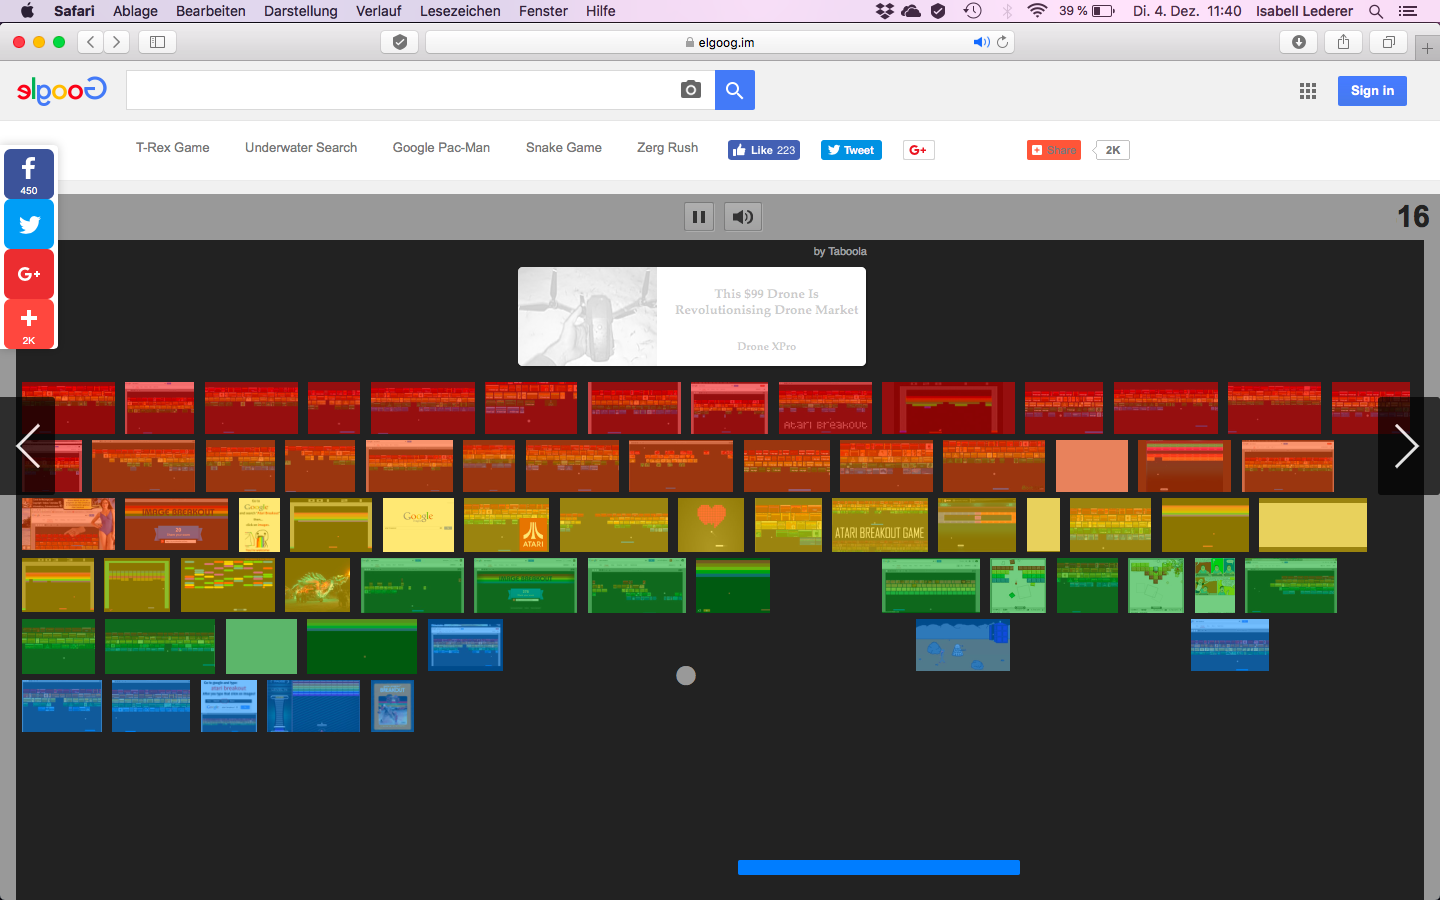
\includegraphics[scale=0.2]{Images/elgoog_breakout}
Breakout at https://elgoog.im/breakout/
\end{frame}
%--------------------------------------------------------------------
\begin{frame}{Some other Atari games}
\begin{columns}
\column{0.5\textwidth}
\centering
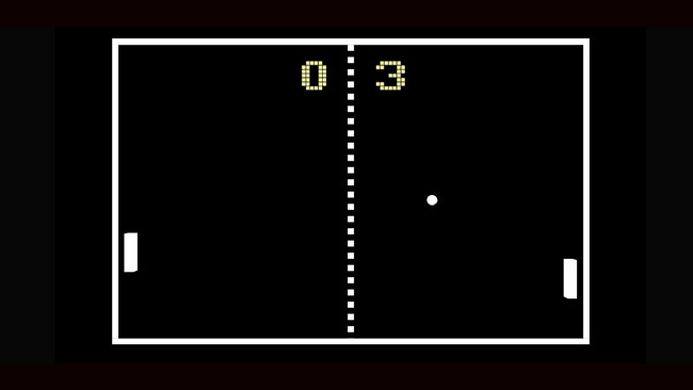
\includegraphics[scale = 0.2]{Images/atari_pong}

\column{0.5\textwidth}
\centering
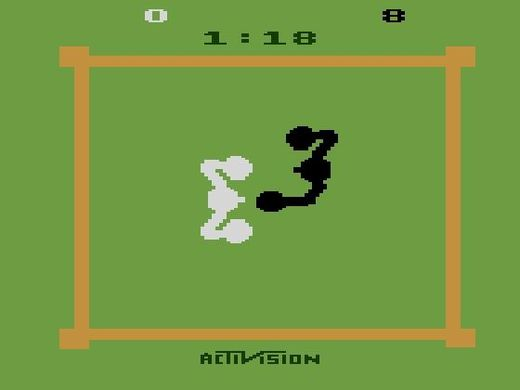
\includegraphics[scale = 0.2]{Images/atari_boxing}
\end{columns}
\vspace*{0.5cm}
\centering
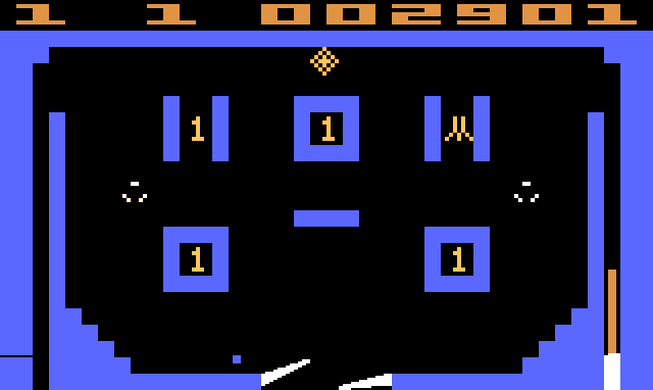
\includegraphics[scale = 0.2]{Images/atari_video-pinball}
\end{frame}
%--------------------------------------------------------------------
\begin{frame}{Reinforcement Learning - Basics}
\begin{textblock}{20}(8,3.5)
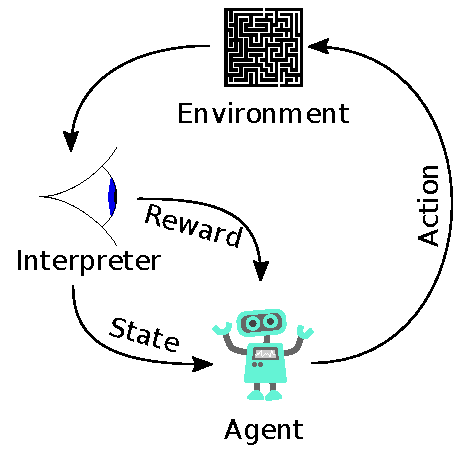
\includegraphics[width = 5cm]{Images/rl_basics.pdf}
\end{textblock}
\end{frame}
%--------------------------------------------------------------------
\begin{frame}{Reinforcement Learning - Basics}

\begin{textblock}{20}(8,3.5)
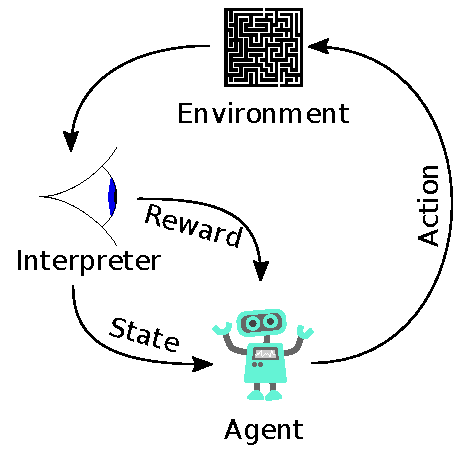
\includegraphics[width = 5cm]{Images/rl_basics.pdf}
\end{textblock}

\begin{textblock}{7}(2,10)
\begin{itemize}

\item {policy function:
	\begin{align*}
	\pi(a\,|\,s)=\mathrm{Pr}(A_t = a \,| \,S_t = s)
	\end{align*}}
\item new problem
\end{itemize}
\end{textblock}
\end{frame}

%--------------------------------------------------------------------
\begin{frame}{The mathematics behind the algorithm}
%\begin{itemize}
\centering
\Large action-value methods vs. policy gradient methods
%\pause
%\item short recap on dynamic dynamic programming
%\end{itemize}
\end{frame}
\begin{frame}{Action-value methods}
methods that approximate an action-value function followed by a policy
\end{frame}
%--------------------------------------------------------------------
\begin{frame}{Action-value methods - Dynamic Programming}
	\begin{itemize}
\item perfect model of environment as Markov Decision Process (MDP)
\pause
\item {dynamics function $p$:
\begin{align*}
p(s',r\,|\,s,a) = \mathrm{Pr}(S_{t} = s', R_t = r\,|\, S_{t-1} = s, A_{t-1} = a)
\end{align*}}
	\end{itemize}
\end{frame}
%--------------------------------------------------------------------
\begin{frame}{Action-value methods - Dynamic Programming}
\begin{itemize}


\item {optimal state-value function $v_*$ and action-value function $q_*$ via Bellmann equations:
\begin{align*}
v_*(s) &= \underset{a}{\mathrm{max}} \; \mathbb{E} \left[ R_{t+1} + \gamma v_* (S_{t+1}) \, | \, S_t = s, A_t = a\right] \\
&= \underset{a}{\mathrm{max}} \sum_{s',r} p(s',r \, | \, s,a) \left[r + \gamma v_*(s')\right],
\\
q_*(s,a) &= \mathbb{E} \left[R_{t+1} + \gamma \, \underset{a'}{\mathrm{max}} q_*(S_{t+1},a') \, |\, S_t = s, A_t = a\right]\\
&= \sum_{s',r} p(s',r \, | \, s,a) \left[r + \gamma \, \underset{a'}{\mathrm{max}} q_* (s',a')\right].
\end{align*}
}
\item characteristic for DP: perfect model as a MDP, approximate optimal value function, bootstrapping
\end{itemize}
\end{frame}
%--------------------------------------------------------------------
\begin{frame}{Action-value methods - Q-learning}
\begin{itemize}
\item {off-policy algorithm that can directly learn from raw experience without a model of the environment's dynamic}
\pause
\item {it has been shown that under some assumptions $Q$ converges with probability $1$ to $q_*$}
\pause
\item {Q-learning iteration:
\begin{align*}
Q(S_t,A_t) \leftarrow Q(S_t, A_t) + \alpha [R_{t+1} + \gamma \, \underset{a}{\mathrm{max}} \, Q(S_{t+1},a) - Q(S_t,A_t)].
\end{align*}}
\end{itemize}
\end{frame}
%--------------------------------------------------------------------
\begin{frame}{Action-value methods - Q-learning Algorithmus}
\begin{exampleblock}{Q-learning Pseudocode}
Parameters: step size $\alpha \in (0,1]$, small $\epsilon > 0$\\
Initialize $Q(s,a)$, for all $s \in \mathcal{S}, a \in \mathcal{A}(s)$, arbitrarily except that $Q(terminal,\cdot) = 0$\\
\vspace*{0.3cm}
Loop for each episode:\\
\hspace*{0.5cm} Initialize S\\
\hspace*{0.5cm} Loop for each step of episode:\\
\hspace*{0.5cm} \hspace*{0.5cm} Choose $A$ by $\epsilon$-greedy selection\\
\hspace*{0.5cm} \hspace*{0.5cm} Take action $A$, observe $R$, $S'$\\
\hspace*{0.5cm} \hspace*{0.5cm} $Q(S,A) \leftarrow Q(S,A) + \alpha \left[ R + \gamma \mathrm{max}_a Q(S',a)-Q(S,A)\right]$\\
\hspace*{0.5cm} until S is terminal
\end{exampleblock}
\end{frame}
%--------------------------------------------------------------------
\begin{frame}{DQN - Deep Q-Network}
\pause
\begin{itemize}
\item combines the idea of Q-learning with a deep convolutional network
\end{itemize}

\centering
\begin{figure}
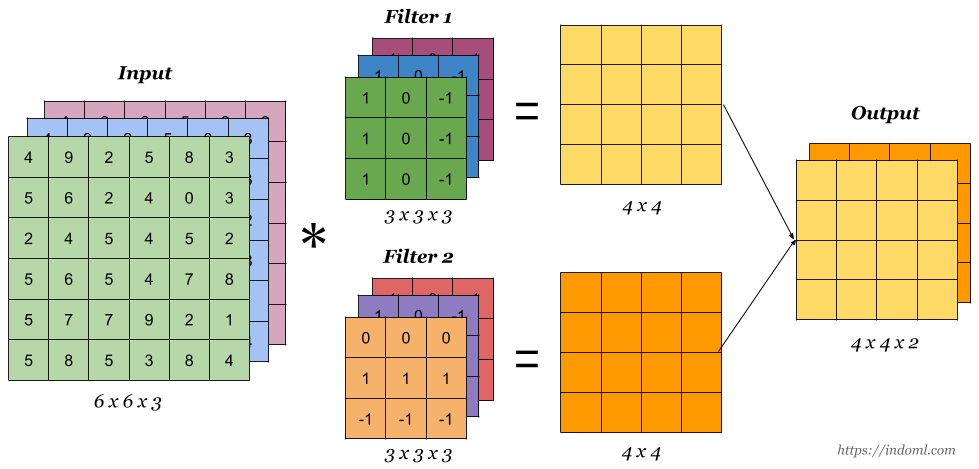
\includegraphics[width = 10cm]{Images/convolution-with-multiple-filters2.png}
\end{figure}
\end{frame}
%--------------------------------------------------------------------
\begin{frame}{Policy Gradient Methods}
\pause
  \begin{itemize}
\item {learn parametrized policy
\begin{align*}
\pi(a\, |\, s, \boldsymbol{\theta}) = \mathrm{Pr}(A_t = a\,|\, S_t= s, \boldsymbol{\theta}_t = \boldsymbol{\theta})
\end{align*}}
\pause
\item learn the parameter $\boldsymbol{\theta}$ based on the gradient of some scalar performance measure $J(\boldsymbol{\theta})$
\pause
\item {updating via gradient ascent
\begin{align*}
\boldsymbol{\theta}_{t+1} = \boldsymbol{\theta}_t + \alpha \widehat{\nabla J(\boldsymbol{\theta}_t)}
\end{align*}}
  \end{itemize}
\end{frame}



%--------------------------------------------------------------------
\begin{frame}{Policy Gradient Methods}
\pause
\begin{itemize}
\item can be parametrized in any way as long as the policy is differentiable
\item to ensure exploration we require that $\pi(a\, |\, s, \boldsymbol{\theta})$ never becomes deterministic
\item {advantage: can approach a deterministic policy
}
\pause
\item one can proof better performance for policy gradient methods than for action value methods
\end{itemize}
\end{frame}

%--------------------------------------------------------------------
\begin{frame}{Policy Gradient Methods}
\begin{itemize}
\item define performance as
\begin{align*}
J(\boldsymbol{\theta}) := v_{\pi_{\boldsymbol{\theta}}}(s_0).
\end{align*}
\pause
\item $\widehat{\nabla J(\boldsymbol{\theta}_t)}$ = ???
\end{itemize}
\end{frame}

%--------------------------------------------------------------------
\begin{frame}{Policy Gradient Theorem}
\begin{theorem}
Let $\pi(a\,|\, s, \boldsymbol{\theta})$ be a parameterized policy, $q_{\pi}(s,a)$ the action-value function under $\pi$ and $\mu(s)$ the on-policy distribution under $\pi$, thus
\begin{align*}
\nabla J(\boldsymbol{\theta}) \propto \sum_s \mu(s) \sum_a q_{\pi}(s,a) \nabla \pi(a\, | \, s, \boldsymbol{\theta}).
\end{align*}

\end{theorem}
\end{frame}
%--------------------------------------------------------------------
\begin{frame}{Policy Gradient Theorem}
\begin{proof}
\renewcommand{\qedsymbol}{}
\begin{align}
\nabla v_{\pi}(s) &= \nabla \Big[\sum_a \pi (a|s) q_{\pi}(s,a) \Big]\\
&= \sum_a \Big[ \nabla \pi(a|s) q_{\pi}(s,a) +  \pi(a|s) \nabla q_{\pi}(s,a) \Big]\\
&= \sum_a \Big[ \nabla \pi(a|s) q_{\pi}(s,a) +  \pi(a|s) \nonumber\\
& \qquad \qquad \qquad \nabla \Big[\sum_{s',r} p(s',r|s,a)\left(r+v_{\pi}(s')\right) \Big]\Big]\\
&= \sum_a \Big[ \nabla \pi(a|s) q_{\pi}(s,a) +  \pi(a|s) \sum_{s'} p(s'|s,a) \nabla v_{\pi}(s') \Big]
\end{align}

\end{proof}
\end{frame}
%--------------------------------------------------------------------
\begin{frame}{Policy Gradient Theorem}
\begin{align*}
(1):\quad & v_{\pi}(s) = \sum_a \pi(s|a)q_{\pi}(s,a)\\
(1) \to (2):\quad & \mathrm{product\; rule}\\
(2) \to (3):\quad & q_{\pi}(s,a) = \sum_{s',r} p(s',r|s,a)\left(r+v_{\pi}(s')\right)\\
(3) \to (4):\quad & p(s'|s,a) = \sum_r p(s',r|s,a)
\end{align*}
\end{frame}
%--------------------------------------------------------------------
\begin{frame}{Policy Gradient Theorem}
\begin{proof}
\vspace*{-0.8cm}
\renewcommand{\qedsymbol}{}
\begin{align}
&= \sum_a \Big[ \nabla \pi(a|s) q_{\pi}(s,a) +  \pi(a|s) \sum_{s'} p(s'|s,a) \nonumber\\
& \qquad  \sum_{a'} \Big[ \nabla\pi(a',s')q_{\pi}(s',a') + \pi(a'|s') \sum_{s''}p(s''|s',a')\nabla V_{\pi}(s'') \Big]\Big]\\
&= \sum_{x \in \mathcal{S}} \sum_{k=0}^{\infty} \mathrm{Pr}(s \to x, k, \pi) \sum_a \nabla \pi(a|x) q_{\pi}(x,a),
\end{align}
where  $\mathrm{Pr}(s \to x, k, \pi)$ is the probability of transitioning from state $s$ to state $x$ in $k$ steps under policy $\pi$.\\
$\eta(s)$ denote the number of time steps spent, on average, in $s$.\\
On-policy distribution is then $\mu(s) = \frac{\eta(s)}{\sum_{s'}\eta(s')}$.
\end{proof}
\end{frame}
%--------------------------------------------------------------------

\begin{frame}{Policy Gradient Theorem}

\begin{proof}
\vspace*{-0.8cm}
\begin{align}
\nabla J(\boldsymbol{\theta}) &= \nabla v_{\pi}(s_0)\\
&= \sum_s \left(\sum_{k=0}^{\infty} \mathrm{Pr}(s_0 \to s, k, \pi) \right) \sum_a \nabla \pi (a|s) q_{\pi}(s,a)\\
&= \sum_s \eta(s) \sum_a \nabla \pi (a|s) q_{\pi}(s,a)\\
&= \sum_{s'} \eta(s') \sum_s\frac{\eta(s)}{\sum_{s'} \eta(s')}  \sum_a \nabla \pi (a|s) q_{\pi}(s,a)\\
&= \sum_{s'} \eta(s') \sum_s \mu(s) \sum_a \nabla \pi (a|s) q_{\pi}(s,a)\\
& \propto \sum_s \mu(s)  \sum_a \nabla \pi (a|s) q_{\pi}(s,a)
\end{align}
\end{proof}

\end{frame}

%--------------------------------------------------------------------
%\begin{frame}{Actor-Critic Methods}
%\centering
%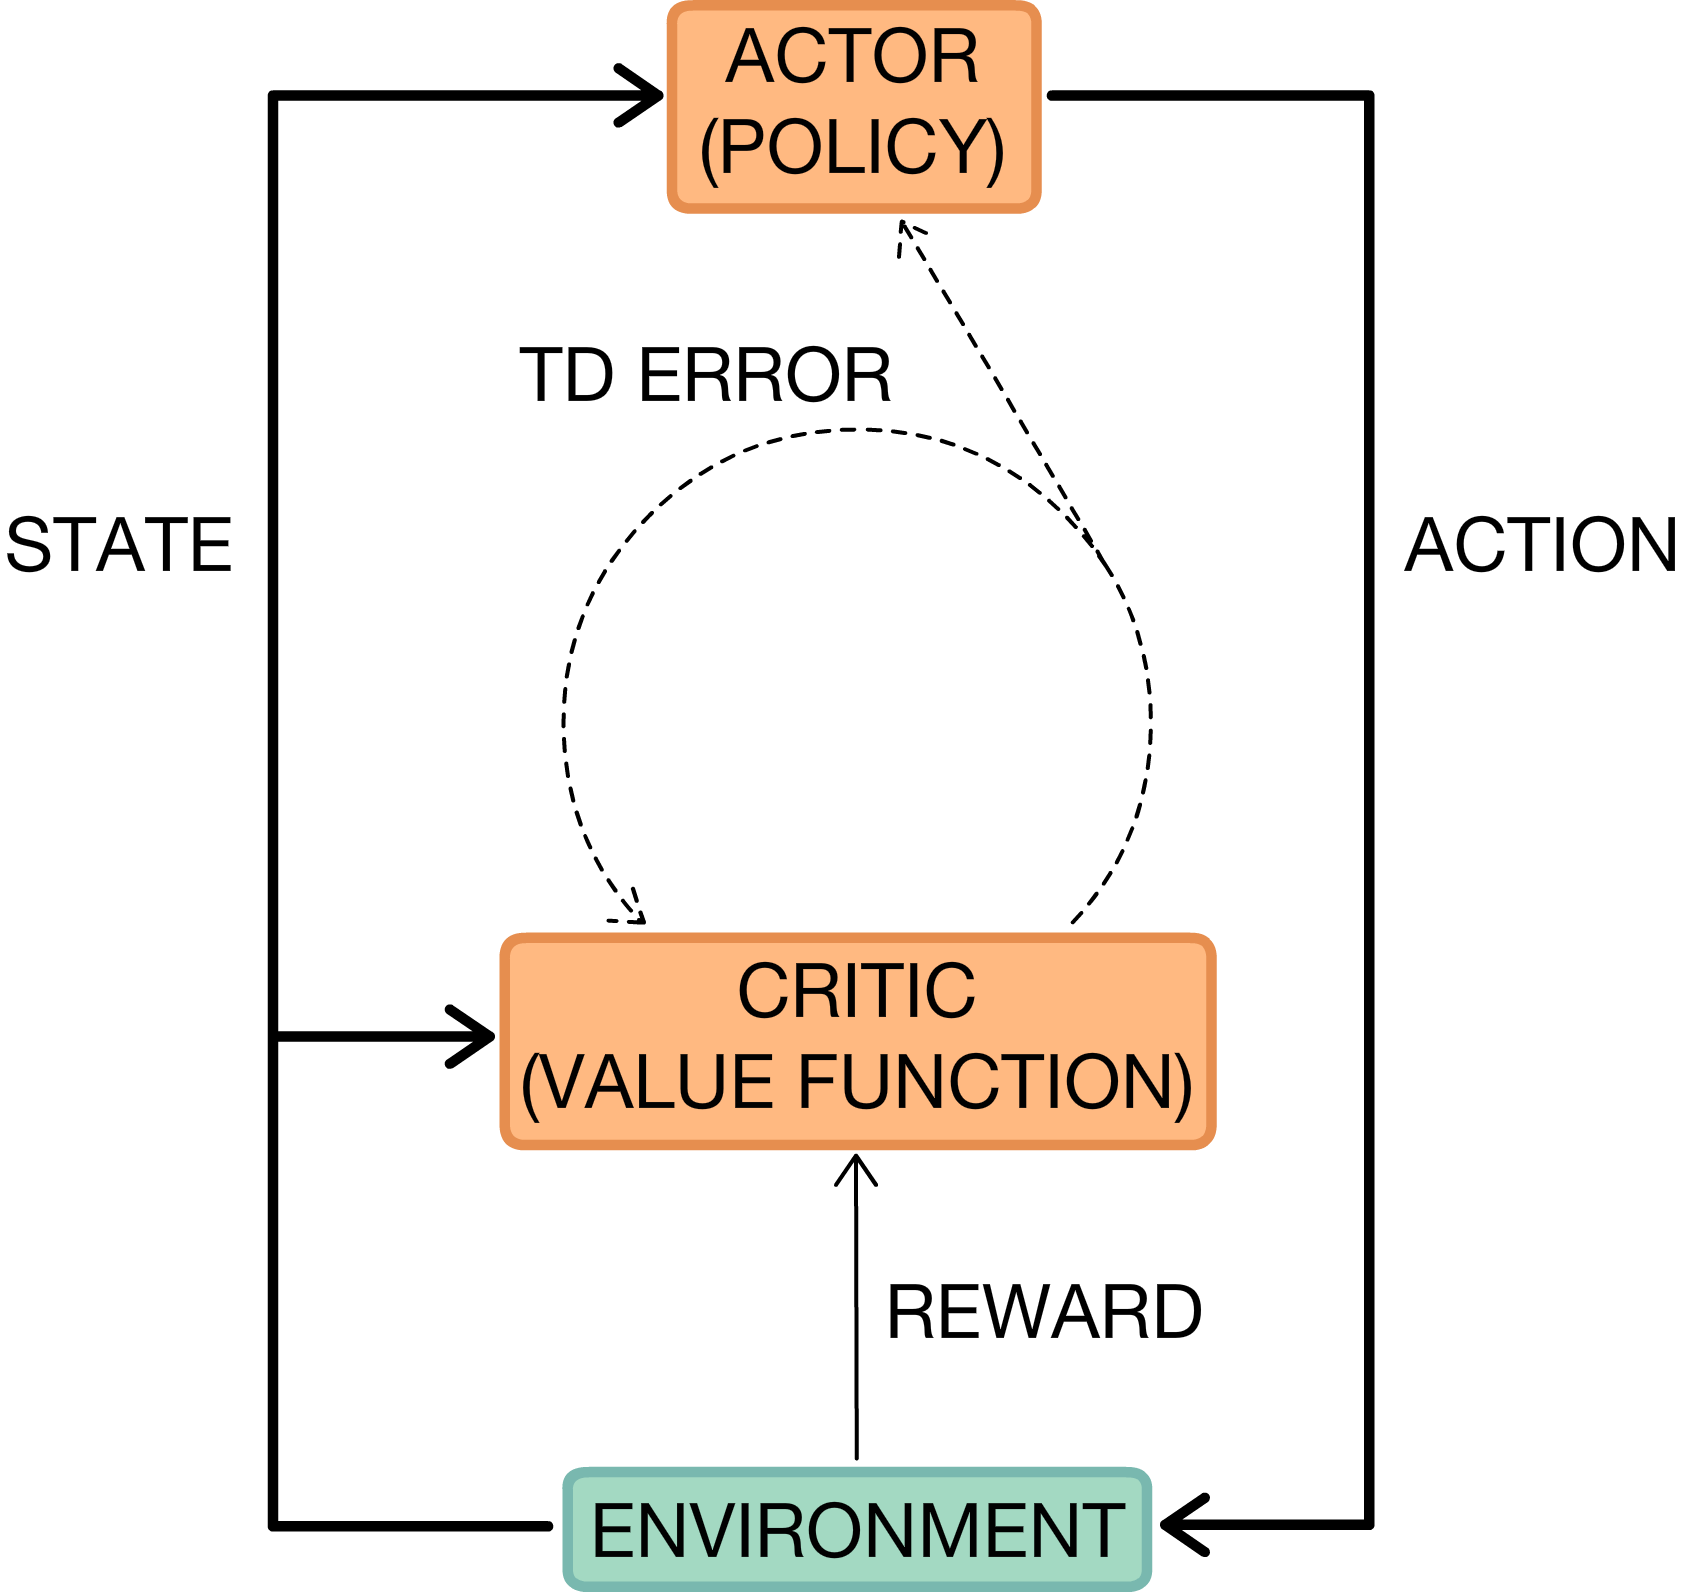
\includegraphics[width = 7cm]{Images/actor-critic.png}
%\tiny https://kaixhin.github.io/deep-reinforcement-learning/actor-%critic.png
%\end{frame}
%--------------------------------------------------------------------
%\begin{frame}{Actor-Critic Methods}
%\begin{itemize}
%\item policy function \textbf{and} value function parametrized
%\pause
%\item {Iteration for one-step Actor-Critic:
%\begin{align*}
%\boldsymbol{\theta}_{t+1} &= \boldsymbol{\theta}_t + \alpha\left(G_{t:t+1} - \hat{v}(S_t, \boldsymbol{\mathrm{w}})\right) \frac{\nabla \pi(A_t\,|\,S_t, \boldsymbol{\theta}_t)}{\pi(A_t\,|\,S_t,\boldsymbol{\theta}_t)}\\
%&= \boldsymbol{\theta}_t + \alpha\left(R_{t+1} + \gamma \hat{v}(S_{t+1}, \boldsymbol{\mathrm{w}})- \hat{v}(S_t, \boldsymbol{\mathrm{w}})\right) \frac{\nabla \pi(A_t\,|\,S_t, \boldsymbol{\theta}_t)}{\pi(A_t\,|\,S_t,\boldsymbol{\theta}_t)}\\
%&= \boldsymbol{\theta}_t + \alpha\, \delta_t\,\nabla \mathrm{ln}\,\pi(A_t\,|\,S_t, \boldsymbol{\theta}_t),
%\end{align*}}
%\pause
%\item big improvement with asynchronous Actor-Critic method
%\end{itemize}
%
%\end{frame}
%--------------------------------------------------------------------
\begin{frame}{Implementation with Python}
\centering

\includegraphics[width = 9cm]{Images/python-logo.png}
\end{frame}
%--------------------------------------------------------------------
\begin{frame}{Emulator}
\begin{itemize}
\item {OpenAI's Gym is a toolkit for developing and comparing reinforcement learning algorithms. It supports teaching agents everything from walking to playing games like Pong or Pinball.}
\pause
\item {Arcade Learning Environment (ALE)}
\end{itemize}
\begin{textblock}{20}(11,3.5)

\includegraphics[scale=0.1]{Images/openAI_logo.png}
\end{textblock}
\end{frame}
%--------------------------------------------------------------------
\begin{frame}{Preprocessing input/images}
	\begin{textblock}{20}(10.5,5)
	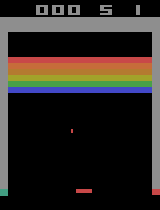
\includegraphics[width = 3.5cm]{Images/breakout_gym.png}
	\end{textblock}
	
	\begin{itemize}
	\item {Input: $3$ Atari frames in $210 \times 160$ pixels\\
	in RGB color}
	\pause
	\item {a lot of data for memory:\\
	memorize recent $1,000,000$ of\\
	($S_t,A_t,R_t,S_{t+1},$\texttt{isTerminal})
	}
	\end{itemize}
\end{frame}
%--------------------------------------------------------------------

\begin{frame}{Preprocessing Input/images}
\begin{itemize}
	\item {Rescaling, e.g. from $210 \times 160$ pixels\\
	to $84 \times 84$}
	\pause
	\item {Greyscaling}	
\end{itemize}

\end{frame}
%--------------------------------------------------------------------
\begin{frame}{Preprocessing Input/images}
	\begin{itemize}
		\item {Rescaling, e.g. from $210 \times 160$ pixels\\
	to $84 \times 84$}
		\item {Greyscaling}
		\begin{textblock}{20}(3,3)
			
\includegraphics[width = 4cm]{Images/skimage_logo}
		\end{textblock}
	\end{itemize}
\end{frame}
%--------------------------------------------------------------------
\begin{frame}{Preprocessing Input/images}
	\begin{itemize}
		\item {Rescaling, e.g. from $210 \times 160$ pixels\\
	to $84 \times 84$}
		\item {Greyscaling}
		\begin{textblock}{20}(3,3)
			
\includegraphics[width = 4cm]{Images/skimage_logo}
		\end{textblock}
		\begin{textblock}{20}(10.5,5)
			
\includegraphics[width = 3.5cm]{Images/breakout_greyscaled}
		\end{textblock}	
	\end{itemize}
\end{frame}
%--------------------------------------------------------------------
\begin{frame}{Storing memory}
\begin{itemize}
\item adequate collection for memory I can sample on
\item deque perfect for needs, but bad runtime
\item implement own RingBuffer?
\end{itemize}

\end{frame}
%--------------------------------------------------------------------
\begin{frame}{Model architecture of DQN}
\centering
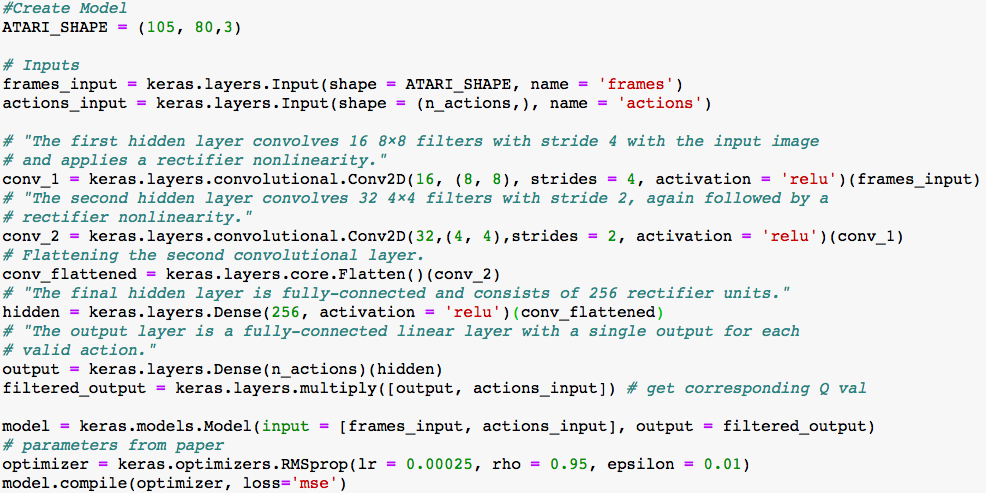
\includegraphics[width = 12cm]{Images/model-code2}
\end{frame}
%--------------------------------------------------------------------

\begin{frame}{Model architecture of DQN}
\centering
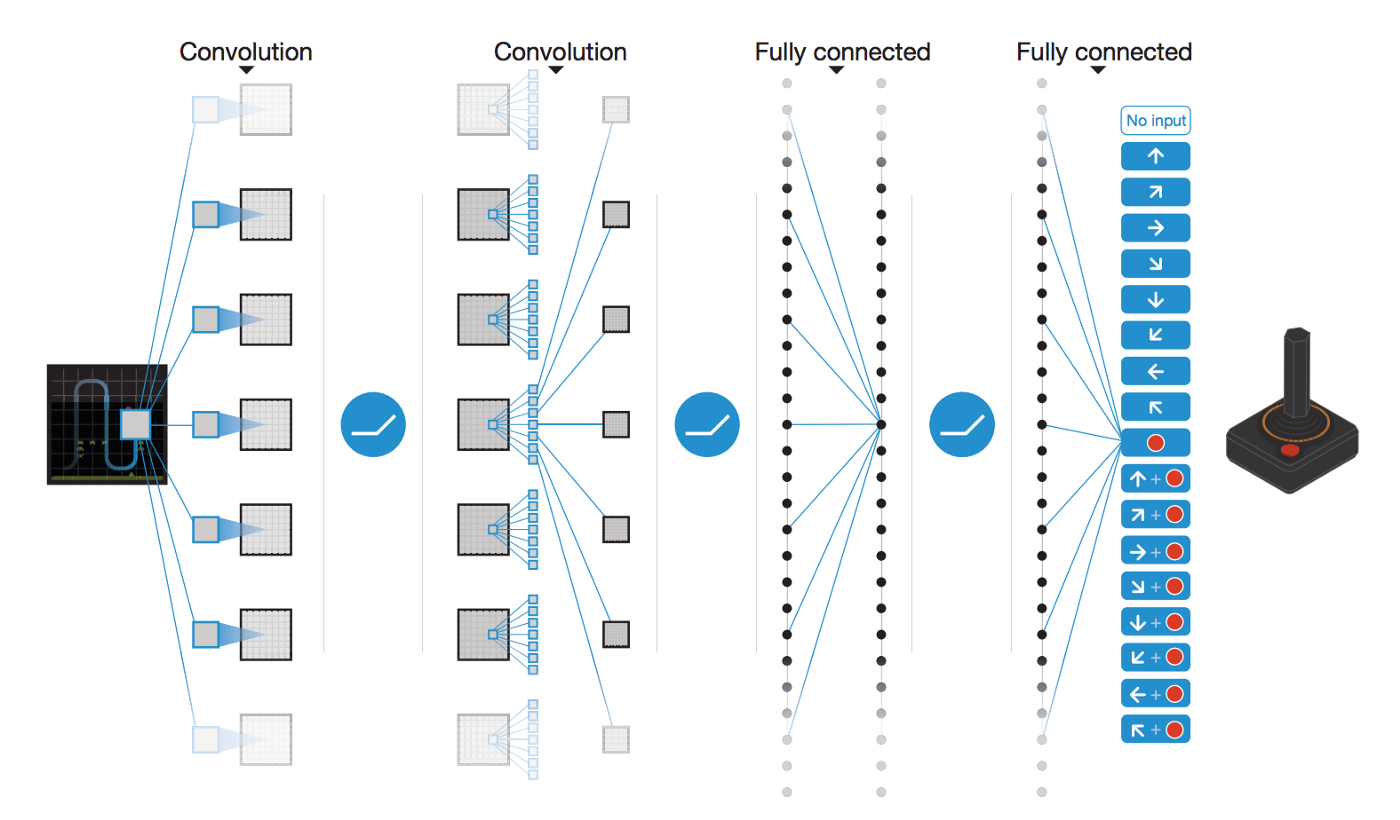
\includegraphics[scale=0.2]{Images/model_architecture.png}
Implementation with \texttt{keras}/ \texttt{tensorflow}
\end{frame}
%--------------------------------------------------------------------
\begin{frame}{Pseudocode DQN}
\begin{exampleblock}{Pseudocode}
\texttt{env = gym.make('BreakoutDeterministic-v4')}\\
Create model, initialize memory $D$\\
Loop for each episode:\\
\hspace*{0.5cm} \texttt{s = env.reset()} and preprocess s\\
\hspace*{0.5cm} \texttt{env.render()}\\
\hspace*{0.5cm} Loop for each step of episode:\\
\hspace*{0.5cm} \hspace*{0.5cm} Choose $\epsilon$, choose with probability $\epsilon$ a random action,\\
\hspace*{0.5cm} \hspace*{0.5cm} otherwise choose best action predicted by model\\
\hspace*{0.5cm} \hspace*{0.5cm} \texttt{s', r, is\_done, info = env.step(a)}\\
\hspace*{0.5cm} \hspace*{0.5cm} preprocess s' and append (s, a, s', is\_done) to $D$\\
\hspace*{0.5cm} \hspace*{0.5cm} sample batch from $D$, predict $Q_{t+1}$, update $Q_t$\\
\hspace*{0.5cm} \hspace*{0.5cm} fit batch of (s,a) with $Q_t$ to model\\
\hspace*{0.5cm}\hspace*{0.5cm} \texttt{env.render()}\\
\hspace*{0.5cm} until $S$ is terminal
\end{exampleblock}
\end{frame}

%--------------------------------------------------------------------
\begin{frame}{Youtube movie of training}
\centering
Video of Playing Atari with Deep Reinforcement Learning:
\url{https://www.youtube.com/watch?v=V1eYniJ0Rnk}
\end{frame}
%--------------------------------------------------------------------
%\begin{frame}{Youtube movie of training}

%\centering After 10 minutes of training
%\center{
%\includemedia[
%  activate=pagevisible,
%  deactivate=pageinvisible,
%  width=270pt,height=150pt,
%]{}{Media/atari_1.swf}
%}\\
%Youtube: Google DeepMind's Deep Q-learning playing Atari Breakout (Two Minute Papers)
%\end{frame}
%--------------------------------------------------------------------
%\begin{frame}{Youtube movie of training}
%\centering After 120 minutes of training
%\center{
%\includemedia[
%  activate=pagevisible,
%   deactivate=pageinvisible,
%  width=270pt,height=150pt,
%]{}{Media/atari_2.swf}
%}\\
%Youtube: Google DeepMind's Deep Q-learning playing Atari Breakout (Two Minute Papers)
%\end{frame}
%--------------------------------------------------------------------
%\begin{frame}{Youtube movie of training}
%\centering After 240 minutes of training
%\center{
%\includemedia[
%  activate=pagevisible,
%    deactivate=pageinvisible,
%  width=270pt,height=150pt,
%]{}{Media/atari_3.swf}
%}\\
%Youtube: Google DeepMind's Deep Q-learning playing Atari Breakout (Two Minute Papers)
%\end{frame}
%--------------------------------------------------------------------
\begin{frame}{Results}
\centering Performance of DQN agent on various Atari games
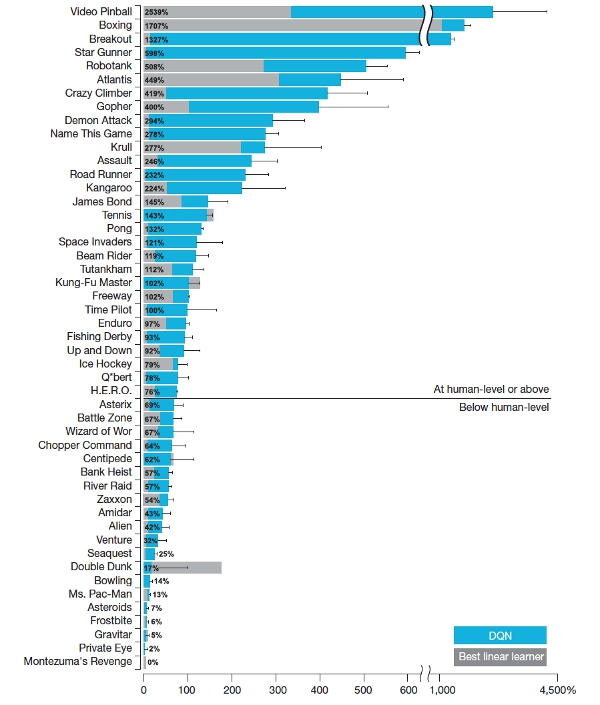
\includegraphics[width = 6.2cm]{Images/deepmind-dqn-perfomance.jpg}
\end{frame}
%--------------------------------------------------------------------
\begin{frame}[focus]
Questions?
\end{frame}
%--------------------------------------------------------------------


% All of the following is optional and typically not needed. 
\appendix
%\section<presentation>*{\appendixname}
%\subsection<presentation>*{Literatur}

\begin{frame}[allowframebreaks]
  \frametitle<presentation>{Literatur}
    
  \begin{thebibliography}{10}
    
  \beamertemplatebookbibitems
  % Start with overview books.

  \bibitem{RLbook}
    R.~S.~Sutton, A.~G.~Barto.
    \newblock {\em Reinforcement Learning - An Introduction}.
    \newblock The MIT Press, 2018.
 
    
  \beamertemplatearticlebibitems
  % Followed by interesting articles. Keep the list short. 

  \bibitem{deepMind}
    Google DeepMind.
    \newblock Human-level control through deep reinforcement learning.
    \newblock {\em Nature}, doi:10.1038/nature14236,
    2015.
  \end{thebibliography}
\end{frame}

\end{document}